\documentclass[tikz,border=5pt]{standalone}
\usepackage{amsmath}
\usetikzlibrary{arrows,calc}

\definecolor{dataBlue}{HTML}{4C78A8}
\definecolor{baselineGray}{HTML}{8C8C8C}
\definecolor{residualAmber}{HTML}{E08E2B}
\definecolor{correctionTeal}{HTML}{2A9D8F}
\definecolor{predictionGreen}{HTML}{59A14F}
\definecolor{charcoal}{HTML}{3A3A3A}

\newcommand{\nodeheader}[1]{%
  {\fontsize{10}{12}\selectfont\bfseries #1}%
}

\begin{document}
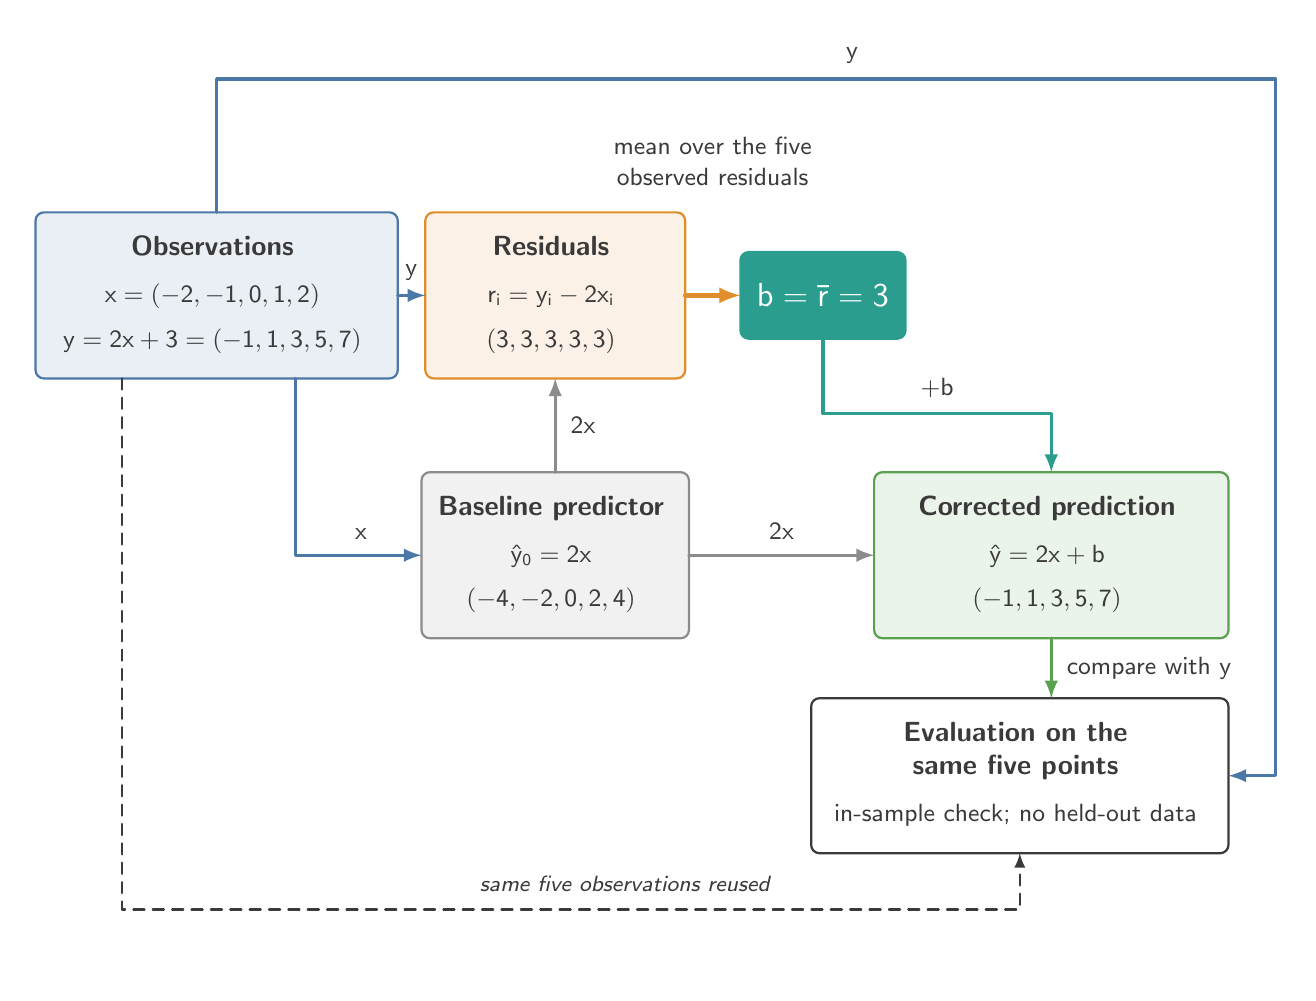
\begin{tikzpicture}[
  font=\sffamily\fontsize{9}{11}\selectfont,
  text=charcoal,
  box/.style={
    rectangle,
    rounded corners=3pt,
    line width=0.8pt,
    inner xsep=6pt,
    inner ysep=8pt,
    align=center,
    outer sep=0pt
  },
  computational/.style={
    -latex,
    line width=1.2pt,
    line cap=round,
    line join=round,
    draw=charcoal
  },
  flowlabel/.style={
    fill=white,
    inner sep=2pt,
    font=\sffamily\fontsize{9}{11}\selectfont
  }
]

% Fixed white canvas: 16 cm by 12 cm, giving a 4:3 aspect ratio.
\path[fill=white] (0,0) rectangle (16,12);
\path[use as bounding box] (0,0) rectangle (16,12);

% Column 1: the five observations.
\node[
  box,
  draw=dataBlue,
  fill=dataBlue!12!white,
  minimum width=4.6cm,
  minimum height=2.1cm
] (D) at (2.4,8.6) {%
  \begin{tabular}{@{}c@{}}
    \nodeheader{Observations}\\[6pt]
    $\mathsf{x=(-2,-1,0,1,2)}$\\[5pt]
    $\mathsf{y=2x+3=(-1,1,3,5,7)}$
  \end{tabular}
};

% Column 2: residuals above the baseline predictor.
\node[
  box,
  draw=residualAmber,
  fill=residualAmber!12!white,
  minimum width=3.3cm,
  minimum height=2.1cm
] (R) at (6.7,8.6) {%
  \begin{tabular}{@{}c@{}}
    \nodeheader{Residuals}\\[6pt]
    $\mathsf{r_i=y_i-2x_i}$\\[5pt]
    $\mathsf{(3,3,3,3,3)}$
  \end{tabular}
};

\node[
  box,
  draw=baselineGray,
  fill=baselineGray!12!white,
  minimum width=3.3cm,
  minimum height=2.1cm
] (B) at (6.7,5.3) {%
  \begin{tabular}{@{}c@{}}
    \nodeheader{Baseline predictor}\\[6pt]
    $\mathsf{\hat{y}_0=2x}$\\[5pt]
    $\mathsf{(-4,-2,0,2,4)}$
  \end{tabular}
};

% Column 3: a single scalar correction.
\node[
  box,
  draw=correctionTeal,
  fill=correctionTeal,
  text=white,
  minimum width=2.05cm,
  minimum height=1.1cm,
  font=\sffamily\fontsize{12}{14}\selectfont
] (S) at (10.1,8.6) {$\mathsf{b=\bar{r}=3}$};

% Column 4: corrected predictions and evaluation.
\node[
  box,
  draw=predictionGreen,
  fill=predictionGreen!12!white,
  minimum width=4.5cm,
  minimum height=2.1cm
] (C) at (13,5.3) {%
  \begin{tabular}{@{}c@{}}
    \nodeheader{Corrected prediction}\\[6pt]
    $\mathsf{\hat{y}=2x+b}$\\[5pt]
    $\mathsf{(-1,1,3,5,7)}$
  \end{tabular}
};

\node[
  box,
  draw=charcoal,
  fill=white,
  minimum width=5.3cm,
  minimum height=1.8cm
] (E) at (12.6,2.5) {%
  \begin{tabular}{@{}c@{}}
    \nodeheader{Evaluation on the}\\[1pt]
    \nodeheader{same five points}\\[6pt]
    in-sample check; no held-out data
  \end{tabular}
};

% A distinct direct target branch into the residuals.
\draw[computational,draw=dataBlue]
  (D.east) -- node[flowlabel,above=3pt] {$\mathsf{y}$} (R.west);

% The input branch drops below the observations before turning right.
\draw[computational,draw=dataBlue]
  ($(D.south)+(1,0)$)
  -- (3.4,5.3)
  -- node[flowlabel,above=3pt,pos=0.52] {$\mathsf{x}$} (B.west);

% Baseline predictions enter the residual calculation from below.
\draw[computational,draw=baselineGray]
  (B.north)
  -- node[flowlabel,right=3pt] {$\mathsf{2x}$} (R.south);

% The observed residuals determine the scalar correction.
\draw[computational,draw=residualAmber,line width=1.6pt]
  (R.east) -- (S.west);

\node[
  align=center,
  text width=3.3cm,
  inner sep=0pt,
  font=\sffamily\fontsize{9}{11}\selectfont
] at (8.7,10.3) {mean over the five\\observed residuals};

% The baseline reaches the corrected predictor horizontally.
\draw[computational,draw=baselineGray]
  (B.east)
  -- node[flowlabel,above=3pt] {$\mathsf{2x}$} (C.west);

% The scalar correction follows an orthogonal route into the top.
\draw[computational,draw=correctionTeal]
  (S.south)
  -- (10.1,7.1)
  -- node[flowlabel,above=3pt] {$\mathsf{+b}$} (13,7.1)
  -- (C.north);

% Corrected predictions are compared with the observed target.
\draw[computational,draw=predictionGreen]
  (C.south)
  -- node[flowlabel,right=3pt] {compare with $\mathsf{y}$}
  (C.south |- E.north);

% A dedicated solid target path follows the top and right perimeter.
\draw[computational,draw=dataBlue]
  (D.north)
  -- (2.4,11.35)
  -- node[flowlabel,above=3pt,pos=0.60] {$\mathsf{y}$} (15.85,11.35)
  -- (15.85,2.5)
  -- (E.east);

% Dashed provenance path: the same observations are reused.
\draw[
  -latex,
  draw=charcoal,
  line width=0.8pt,
  dash pattern=on 4pt off 3pt,
  line cap=round,
  line join=round
]
  ($(D.south)+(-1.2,0)$)
  -- (1.2,0.8)
  -- node[
    flowlabel,
    above=4pt,
    pos=0.56,
    font=\sffamily\fontsize{8}{10}\selectfont\itshape
  ] {same five observations reused} (12.6,0.8)
  -- (E.south);

\end{tikzpicture}
\end{document}